%%%%%%%%%%%%%%%%%%%%%%%%
% Sample use of the infthesis class to prepare an MSc thesis.
% This can be used as a template to produce your own thesis.
% Date: June 2019
%
%
% The first line specifies style options for taught MSc.
% You should add a final option specifying your degree.
% *Do not* change or add any other options.
%
% So, pick one of the following:
% \documentclass[msc,deptreport,adi]{infthesis}     % Adv Design Inf
% \documentclass[msc,deptreport,ai]{infthesis}      % AI
% \documentclass[msc,deptreport,cogsci]{infthesis}  % Cognitive Sci
% \documentclass[msc,deptreport,cs]{infthesis}      % Computer Sci
% \documentclass[msc,deptreport,cyber]{infthesis}   % Cyber Sec
% \documentclass[msc,deptreport,datasci]{infthesis} % Data Sci
% \documentclass[msc,deptreport,di]{infthesis}      % Design Inf
% \documentclass[msc,deptreport,inf]{infthesis}     % Informatics
%%%%%%%%%%%%%%%%%%%%%%%%

\documentclass[mphil,deptreport,ai]{infthesis} % Do not change except to add your degree (see above).
\usepackage[final]{pdfpages}

\begin{document}
\begin{preliminary}

\title{Spiking neural network model construction, inference, analysis and application}

\author{William Peer Berg}

\abstract{
%   Lorem ipsum. More computational power. More data, and higher res. data available. Modelling may (1) explain aspects about recorded site(s), and (2) generate hypotheses that may be tested with in vivo recording.
%   However, inference of high-dimensional biologically realistic (to some extent) models NP-hard, computationally costly, does not scale well with growing resolution due to dimensionality and cost, and not automated. Often experts are required to make an effort at hand-engineering models for particular data. As such, model inference of biologically realistic/plausible models is a highly challenging task, which if more automated might be of great benefit to the field of computational neuroscience.
%   Looking to machine learning and the success in applying gradient-based optimisation to tackle high-dimensional modelling problems, we here investigate the potential of applying this to the class of spiking neural network models. Further, we look at statistical assessment methods, and application of outlined methodology both to synthetically generated as well as biologically recorded in vivo data.
%   In sum, our results show that models may capture higher-order statistics of recorded nuclei, and that using some parallelisation tricks, we may decrease the computational cost to some extent. However, the lower bound on computational complexity still makes it challenging to apply the outlined methodology to very rich (i.e. high number of recorded nuclei) data sets.
SNNs biologically realistic models. Do we have the tools for SNN parameter inference, instead of rigorous and tedious hand-engineering?
ML advances: GBO.
SNNs differ from RNNs in a fundamental/crucial way. Show via parameter landscape and loss functions.
However, can find frontier(s).
SNN variants and applicability of GBO (only NLIF thus far, but still local minima).
To some extent GIF; frontier.
Same for GLIF versions??
Input scheme. Param landscape plots.
Loss functions.
PyTorch (+batching)

ABC, (EA; e.g. NGO)

Albeit GT off for the above, comparison wrt NMF.
Hand-engineered case and full analysis with NMF and LDA.

In conclusion...

BONUS (if time): Fitting to sleep data, with small sleep regul PPT/LDT lit rev first?

BONUS2: Append Izhikevich paper and place in context.

BONUS3: ?
}

\maketitle

\section*{Acknowledgements}
Arno.
Nina.
Patricia.
Luke.
Matthias.
Shuzo.

\tableofcontents
\end{preliminary}


\chapter{Introduction}


% The report then contains a bibliography and any appendices, which may go beyond
% page~40. The appendices are only for any supporting material that's important to
% go on record. However, you cannot assume markers of dissertations will read them.

% Citations (such as \cite{P1} or \cite{P2}) can be generated using
% \texttt{BibTeX}. For more advanced usage, the \texttt{natbib} package is
% recommended. You could also consider the newer \texttt{biblatex} system.

% You may not change the dissertation format (e.g., reduce the font
% size, change the margins, or reduce the line spacing from the default
% 1.5 spacing). Over length or incorrectly-formatted dissertations will
% not be accepted and you would have to modify your dissertation and
% resubmit.  You cannot assume we will check your submission before the
% final deadline and if it requires resubmission after the deadline to
% conform to the page and style requirements you will be subject to the
% usual late penalties based on your final submission time.

Spiking neural networks (SNNs) contain variables that represent biological properties such as membrane potential, temporal signature, and potentially ion channel dynamics. Their definition results in membrane voltage dynamics resembling that of biological neurons, including the release of action potentials upon reaching a certain membrane potential.
Due largely to the biological plausibility of this class of neural network models, they are appealing to study in computational neuroscience, as they may trail biology to a greater extent than the feed-forward networks as often seen in the machine learning domain.
However, training SNNs is yet of limited success, and model inference also faces a number of challenges due to the temporal constraints introduced by SNNs, as well as the increased complexity of this model class.
We here revisit the state-of-the art for inferring SNN models using both surrogate gradient based optimisation and some of the most prominent spike metrics, as well as deep neural network amortized learning and approximate Bayesian computation (ABC), and compare how these approaches may be employed for SNN inference. Further, we hypothesise that recent ML techniques may be leveraged for successful and efficient model inference using surrogate gradient descent.
We find that while ABC may be successful for population-level models, as has been shown recently in the literature, its algorithmic and computational complexity and cost thereof limits the methodology to a low number of nodes, particularly for more high-dimensional leaky integrate-and-fire (LIF) model extensions.
However, using a surrogate gradient approach, we find that model inference for larger networks is made possible. We perform model inference using a set of LIF-extensions, leading up to the GLIF model using (both) synthetic (and biological) data, and demonstrate that higher order statistics may be captured (to some extent) even when performing neuron-level model inference over a mixed neuron-type network.
This may advance research on SNN inference, and also demonstrates how modern ML frameworks as well as techniques may be leveraged to this end.

\chapter{Background}

% 1: Something you can learn about network, but also should be specific to a spiking net
% Want to find something only in SNN, but which is also identifiable
% Don’t need to find exact same sync act., not same identities of neurons which participate, just general properties, in spite of unknown input activity

% No model inputs
% We can say something about the state - or if we can: Could this be used to constrain parameter search? Could it make the van Rossum distance better than the mean firing rate distance?

Include LIF paper draft and report.

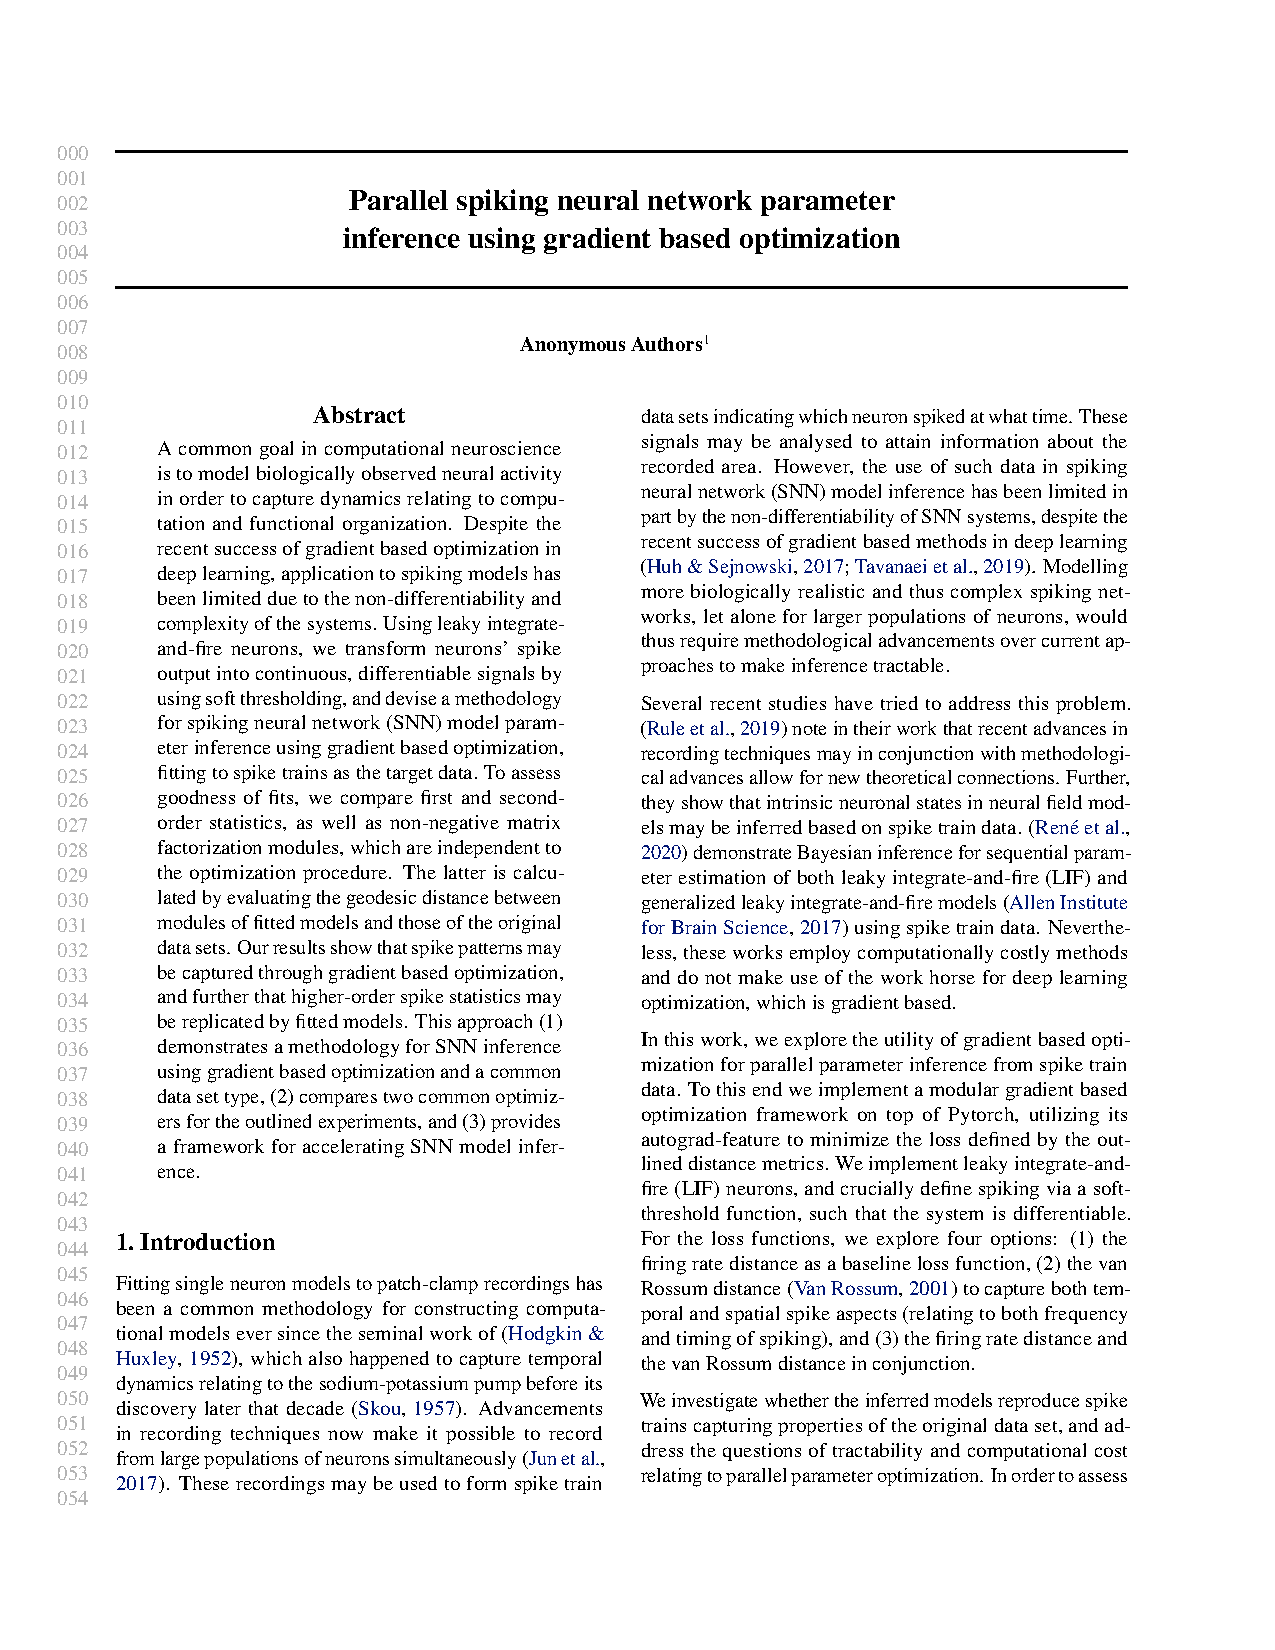
\includepdf[pages=-]{files/icml2021_draft_snn_inference.pdf}

\cite{Lueckmann2018} amortised learning and ABC using DNNs.

\cite{Taherkhani2020} learning in SNNs

\cite{Rene2020} "special case" i.e. mesoscopic-microscopic inference using first ABC (or GD?) on pop. level and then MCMC sampling for full approx. posterior?


\bibliographystyle{plain}
\bibliography{references}

%% You can include appendices like this:
% \appendix
% 
% \chapter{First appendix}
% 
% \section{First section}
% 
% Markers do not have to consider appendices. Make sure that your contributions
% are made clear in the main body of the dissertation (within the page limit).

\end{document}
